\chapter{Fine-Tuning Methodology and Optimizers}

\vspace*{0.3cm}

The fine-tuning methodology adapts \texttt{google/flan-t5-small} \cite{flant5}
to the prepared
instruction-following dataset. The tokenizer converts \texttt{source\_text} and
\texttt{target\_text} into token IDs using padding and truncation. The training
script then loads the model, selects the optimizer, runs the training loop,
evaluates the model, and saves the metrics.

\begin{figure}[H]
    \centering
    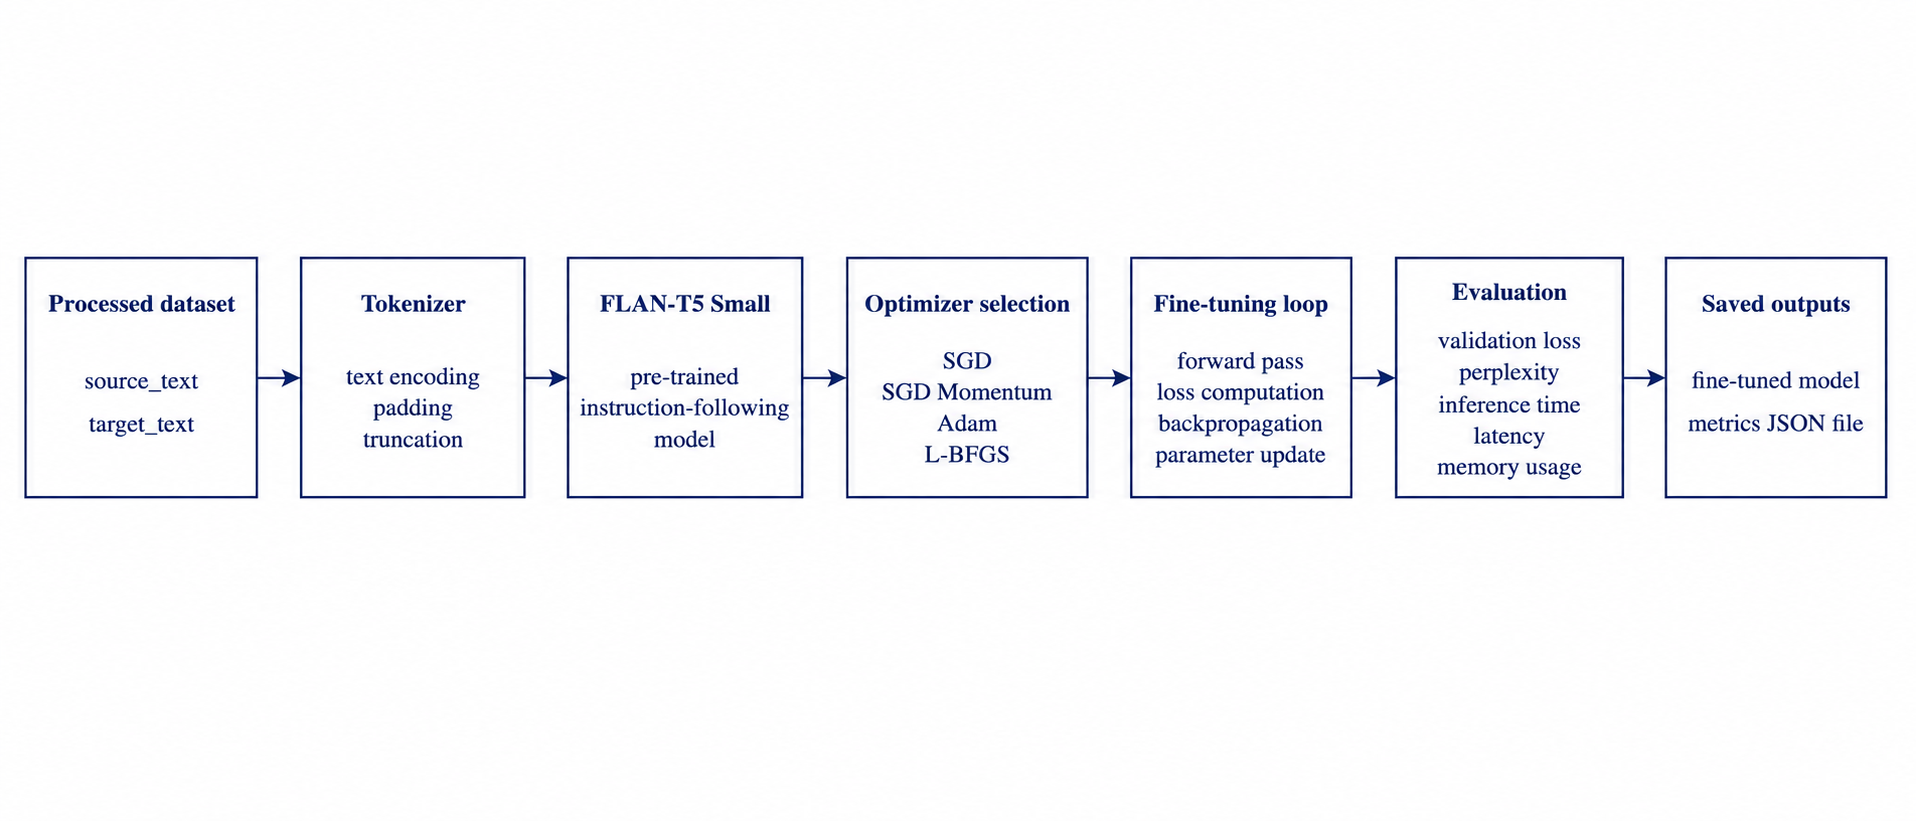
\includegraphics[width=\textwidth]{chapters/images/finetunning_flow.png}
    \caption{Fine-tuning workflow used in the project.}
    \label{fig:finetuning_workflow}
\end{figure}

The main implementation is organized around \texttt{src/train.py}, supported by
\texttt{model\_utils.py}, \texttt{tokenizer\_utils.py}, \texttt{optimizers.py},
\texttt{training\_config.py}, and \texttt{metrics.py}. The implementation relies
on the Hugging Face Transformers ecosystem \cite{transformers}. The experiments were run
on a CUDA-enabled GPU, specifically an RTX 5060. CPU execution is kept only for
debugging because it is too slow for complete optimizer comparison.

\begin{figure}[H]
    \centering
    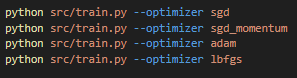
\includegraphics[width=0.5\textwidth]{chapters/images/optimizer_training_commands.png}
    \caption{Commands used to launch fine-tuning with each optimizer.}
    \label{fig:optimizer_training_commands}
\end{figure}

SGD is the simplest first-order method and updates parameters using the gradient
of the loss \cite{sgd}.

\[
\theta_{t+1} = \theta_t - \eta \nabla_{\theta} L(\theta_t)
\]

It is memory-efficient but can converge slowly. SGD with momentum improves this
method by accumulating part of the previous update direction, which reduces
oscillation and can accelerate convergence.

\[
v_{t+1} = \mu v_t + \nabla_{\theta}L(\theta_t), \quad \theta_{t+1} = \theta_t - \eta v_{t+1}
\]

Adam, or Adaptive Moment Estimation, combines momentum and adaptive learning
rates by maintaining moving averages of gradients and squared gradients. It is
widely used for transformer fine-tuning because it often reduces loss faster than
SGD \cite{adam}.

\[
m_t = \beta_1m_{t-1} + (1-\beta_1)g_t, \quad v_t = \beta_2v_{t-1} + (1-\beta_2)g_t^2, \quad \theta_{t+1} = \theta_t - \eta\frac{\hat{m}_t}{\sqrt{\hat{v}_t}+\epsilon}
\]

AdamW extends Adam by decoupling weight decay from the gradient
update, which can improve regularization \cite{adamw}.

\[
\theta_{t+1} = \theta_t - \eta\left(\frac{\hat{m}_t}{\sqrt{\hat{v}_t}+\epsilon} + \lambda\theta_t\right)
\]

L-BFGS is a quasi-Newton method that
approximates curvature information but is expensive for transformer models
\cite{lbfgs}.

\[
p_k = -H_k \nabla_{\theta}L(\theta_k), \quad \theta_{k+1} = \theta_k + \alpha_k p_k
\]

Newton-CG is a second-order method based on Hessian information; it is useful for
academic comparison but costly in practice.

\[
\theta_{t+1} = \theta_t - H^{-1}\nabla_{\theta}L(\theta_t)
\]

Each optimizer saves its own model under \texttt{results/models/} and its metrics
under \texttt{results/metrics/}. This makes the comparison reproducible and keeps
the outputs of each experiment separated.
